\documentclass{standalone}
\usepackage{tikz}
\usepackage{ctex,siunitx}
\setCJKmainfont{Noto Serif CJK SC}
\usepackage{tkz-euclide}
\usepackage{amsmath}
\usetikzlibrary{patterns, calc,3d}
\usetikzlibrary {decorations.pathmorphing,decorations.pathreplacing,decorations.shapes}
\tikzset{label style/.append style={font=\small}}
\begin{document}
\small
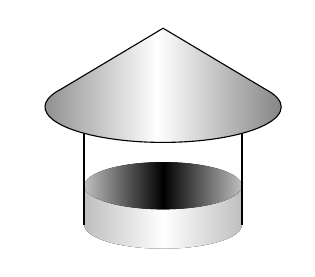
\begin{tikzpicture}[>=latex,scale=1.0]
  \fill[left color=lightgray,right color =lightgray,middle color=white](1,0)arc(0:-180:1 and 0.3)--(-1,0.5)--(1,0.5);
  \fill[left color=lightgray,right color =lightgray,middle color=black](0,0.5)ellipse(1 and 0.3);
  \draw[thick](-1,0)--(-1,1.5)(1,0)--(1,1.5);
  \draw[left color=gray,right color=gray,middle color=white]({1.5*cos(150)},{1.5+0.45*sin(150)})arc(150:390:1.5 and 0.45)--(0,2.5)--cycle;
\end{tikzpicture}
\end{document}